\documentclass[12pt,a4paper]{article}
\usepackage[utf8]{inputenc}
\usepackage[spanish]{babel}
\usepackage{amsmath}
\usepackage{amsfonts}
\usepackage{amssymb}
\usepackage{amsthm}
\usepackage{graphicx}
\usepackage[left=2cm,right=2cm,top=2cm,bottom=2cm]{geometry}
\title{Practica 1 - TALF}
\author{José Antonio Luque Salguero}
\date{}
\setlength{\parindent}{0pt}
\begin{document}

\newtheorem*{definicion}{Definición}

\maketitle

1. Encuentra el conjunto potencia del conjunto $ \mathcal{R}^{3} $ de $\mathcal{R} = \{ (1,1), (1,2), (2.3), (3,4) \}$.
 Comprueba tu respuesta con el script \textbf{powerrelation.m} y escribe un documento \LaTeX con la solución paso por paso.

 \vspace*{4mm}

En primer lugar observemos la definición de conjunto potencia:

\begin{definicion}[Conjunto potencia] 
Dado $\mathcal{R} \subset A \times A $

\[ 
  \mathcal{R}^{n}= \begin{cases} 
    \mathcal{R} & n=1 \\
    \{ (a,b): \exists x \in A, (a,x) \in \mathcal{R}^{n-1} \wedge (x,b) \in \mathcal{R} \} & n>1
  \end{cases}
\]
\end{definicion}

Como podemos ver se trata de una definicion recursiva, calculemos entonces $\mathcal{R}^2$.

\[
  \mathcal{R}^{2} = \{ (a,b): \exists x \in A, (a,x) \in \mathcal{R}  \wedge (x,b) \in \mathcal{R} \} = \{ (1,1),(1,2), (1,3),(2,4)\}  
\]

Finalmente calculemos  $\mathcal{R}^3$.
\[
  \mathcal{R}^{3} = \{ (a,b): \exists x \in A, (a,x) \in \mathcal{R}^2  \wedge (x,b) \in \mathcal{R} \} = \{ (1,1),(1,2),(1,3),(1,4)\}  
\]

Comprobemos que solución encontrada es correcta comparandola con la proporcionada por el scritp \textbf{powerrelation.m}.
\begin{figure}[h]
\centering
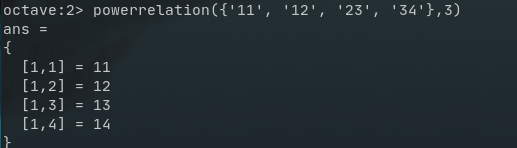
\includegraphics{2021-10-17_15-14.png}
\end{figure}

\end{document}

